\cotefile{157-4}
\scanpage{132}
\mspage{6}
% archive sheet number: 131
(1.16.) Les flèches $i\in C_0$ sont \unsure{co-quarrables}, i.e. pour un diagramme
\diagram{\begin{tikzcd}[ampersand replacement=\&]
A \arrow[r,dash,"u"] \arrow[d,"i"'] \& X \\
B \&
\end{tikzcd}}
avec $i\in C_0$, la somme \unsure{amalgamée} existe.

Mais on peut formuler (1.15) aussi ainsi, indépendamment de l'hypothèse (1.16.) :

(1.1\deleted{\unsure{5|6}}7 \unsure{bis}) Pour \unsure{tt} \unsure{diagramme}
\diagram{\begin{tikzcd}[ampersand replacement=\&]
A \arrow[r,dash,"u"] \arrow[d,"i"'] \& X \arrow[d,"f"] \\
\unsure{B} \arrow[r,"\unsure{v|\nu}"'] \& Y
\end{tikzcd}}
, avec $i\in C_0$, existe \deleted{\unsure{de $f$}} un carré comm. traits pleins
\diagram{\begin{tikzcd}[ampersand replacement=\&]
A \arrow[r,phantom,"\unsure{-|\to}" description,"u"] \arrow[d,"i"'] \& X \arrow[d,"i_1(f)"] \\
B \arrow[r,"v_1"] \arrow[dr,dashed,"v"'] \& X_1(f) \arrow[d,dashed,"p_1(f)"] \\
\& Y
\end{tikzcd}}
tel que $v=p_1(f)v_1$.

Ceci a pour conséquence le
\uline{Corollaire 1} \inserted{(de 1.17)} \inserted{Soit $f\in\mathrm{Fl}\,M$, et} \inserted{$\alpha$ un ordinal $(\in\unsure{\mathcal U|U})$,}
Pour \unsure{tout|tt} \deleted{diagramme}\inserted{carré} commutatif
\diagram{\begin{tikzcd}[ampersand replacement=\&]
A \arrow[r,"\unsure{u_\alpha|u}"] \arrow[d,"i"'] \& X_\alpha(f) \arrow[d,"p_\alpha(f)"] \\
B \arrow[r,"v"'] \& Y
\end{tikzcd}}
il existe un carré commutatif
\diagram{\begin{tikzcd}[ampersand replacement=\&]
A \arrow[r,phantom,"\unsure{\to|-}" description,"u_\alpha"] \arrow[d] \& X_\alpha(f) \arrow[d,"\operatorname{trans}"] \arrow[dd,bend left=45,dashed,"p_\alpha(f)"] \\
B \arrow[r,"v_1"] \arrow[dr,dashed,"v"'] \& X_{\alpha+1}(f) \arrow[d,phantom,"\unsure{\vert|\downarrow}" description,"p_{\alpha+1}(f)"] \\
\& Y
\end{tikzcd}}
tel que
\[v=p_{\alpha+1}(f)v_1.\]

\scanpage{133}\mspage{7}
% archive sheet number: 132
\uline{Corollaire 2} Soit $\unsure{I|\pi}$ un cardinal $(\in\unsure{\mathcal U|U})$ tel que pour toute \deleted{$i\in C_0$, la source} $i:A\to B$ dans $C_0$, la source $A$ soit $\pi$-admissible. Soit $\alpha$ un ordinal grand devant $\pi$ (i.e. tel que l'ensemble \inserted{\unsure{noté|notons} $I_\alpha$} des ordinaux $\alpha'<\alpha$ soit grand devant $\pi$) -- p.ex. $\alpha$ le premier ordinal dont le cardinal soit $>\pi$. Alors pour tout $f\in\mathrm{Fl}(M)$, \inserted{\unsure{on a}} $p_\alpha(f)\in C_{0*}$.

\uline{\unsure{Dém|Dèm}} Cela signifie que pour \unsure{tt} carré comm.
\diagram{\begin{tikzcd}[ampersand replacement=\&,column sep=large,row sep=large,execute at end picture={\node[anchor=east] at ([xshift=-45pt]current bounding box.west) {$\unsure{(\alpha)|(a)}$};\node[anchor=west] at ([xshift=25pt]current bounding box.east) {, avec $i\in C_0$,};}]
A\arrow[r,"u"]\arrow[d,dash,"i"']\&X_\alpha(f)\arrow[d,"p_\alpha(f)"]\\
B\arrow[r,"v"']\arrow[ur,dotted,"w"]\&Y
\end{tikzcd}}
la flèche pointillée $w$ (avec $wi=u$, $p_\alpha(f)w=v$) existe.

Or $X_\alpha(f)=\varinjlim_{\alpha'\in I_\alpha}X_{\alpha'}(f)$, avec \deleted{$A$} $A$ est $\pi$-acc. et $I_\alpha$ grand devant $\pi$, $u$ provient d'une flèche $u_{\alpha'}:A\to X_{\alpha'}(f)$, et quitte à remplacer $\alpha'$ par $\alpha''>\alpha'$ et $u_{\alpha'}$ par le composé $u_{\alpha''}:A\mathbin{-}X_{\alpha'}(f)\to X_{\alpha''}(f)$) \deleted{\unsure{on a|on}} $p_{\alpha'}(f)u_{\alpha'}=vi$, i.e. qui \deleted{\unsure{colle}} \inserted{provient} d'un carré commutatif
\diagram{\begin{tikzcd}[ampersand replacement=\&,column sep=large,row sep=large]
A\arrow[r,"u_{\alpha'}"]\arrow[d,dash,"i"']\arrow[rr,bend left=24,dashed,"u_\alpha"]\&X_{\alpha'}(f)\arrow[r,dashed,"\mathrm{trans}"']\arrow[d,"p_{\alpha'}(f)"]\&X_\alpha(f)\arrow[dl,dashed,"p_\alpha(f)"]\\
B\arrow[r,dash,"v"]\&Y\&
\end{tikzcd}}
, et appliquant le cor. 1, on trouve
\diagram{\begin{tikzcd}[ampersand replacement=\&,column sep=large,row sep=large]
A\arrow[r,dash,"\unsure{u_{\alpha'}|u_{\alpha''}}"]\arrow[d,dash]\&X_{\unsure{\alpha'|\alpha''}}(f)\arrow[d,"\mathrm{trans}."]\&\\
B\arrow[r,dash,"v_1"]\arrow[dr,dashed,"v"']\&X_{\alpha'\unsure{+|-}1}(f)\arrow[r,dashed,phantom,"\unsure{-|\to}"description,"\mathrm{trans}"]\arrow[d,"p_{\alpha'+1}(f)"]\&X_\alpha(f)\arrow[dl,dashed,"p_\alpha(f)"]\\
\&Y\&
\end{tikzcd}}
avec $v=p_{\alpha'+1}(f)v_1$, et on prendra
\[
w=\mathrm{trans}_{\alpha,\alpha'+1}\circ v_1.
\]

\scanpage{134}\mspage{8}
% archive sheet number: 133 (upper left)
Mais on veut une factorisation de $f$, flèche quelconque dans $M$ en
\[
f=pi,\quad\text{avec }p\in C_{0*}\quad\uuline{\text{et}}\quad i\in\widetilde C_0,
\]
donc il faut encore \unsure{énoncer} une propriété, assurant que les $i_\alpha(f)$ sont dans $\unsure{\widetilde C_0|\widetilde C}$. On aura $\unsure{\simeq|=}$ quelque \unsure{chose} de plus précis. Introduisons donc
\[
\begin{aligned}
C'_0={}&\text{plus petit sous-ensemble de }\mathrm{Fl}\,M\\
&\text{contenant }C_0,\text{ stable par cochangement de}\ \deleted{\unsure{petites}}\\
&\text{base (chaque fois qu'il existe),}\ \deleted{\unsure{et par}}
\end{aligned}\tag*{1.18.}
\]
\[
\begin{aligned}
C''_0={}&\deleted{\text{\unsure{ensemble des sommes amalgamées de flèches}}}\ \inserted{\text{\unsure{flèches qui sont soit}}}\\
&\text{dans }C'_0,\text{ soit des sommes amalgamées}\\
&\inserted{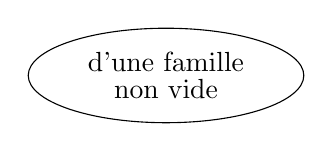
\begin{tikzpicture}[baseline=(t.base)]
\node[inner sep=2pt] (t) {\shortstack{d'une famille\\non \uuline{vide}}};
\draw (t.center) ellipse (1.75cm and .6cm);
\end{tikzpicture}}\quad\text{\unsure{telles flèches}}\ \deleted{\text{\unsure{de flèches}}}\quad A\xrightarrow{i_\alpha}B_\alpha\\
&\text{de }\unsure{\simeq|=}\text{ source }\inserted{A},\quad i_\alpha\in C'_0;\text{ la flèche}\\
&A\longrightarrow B=\coprod_{\alpha\,(A)}B_\alpha\quad\text{est dans }C'_0.
\end{aligned}
\]
% slanted; crossed block in the left margin
\margin{\deleted{\deleted{\unsure{Variante|Voir note|Vérifier}} \uline{NB} \unsure{Il n'est pas sûr que} les $i\in C''_0$ soient \unsure{quarrables}, si les \unsure{changements} de base \illegible{4} \unsure{Remarqué d'ici}.}}

(La condition 1.16. implique que les éléments de $C'_0$ sont \unsure{coquarrables}, et cela suffit, avec la condition de stabilité de $M$ par \deleted{\unsure{petites}} $\varinjlim$ filtrantes, à assurer que les sommes amalgamées infinies envisagées \deleted{\unsure{sont bien}} existent dans $M$.)
\[
\begin{aligned}
C'''_0={}&\text{plus petit sous-ensemble de }\mathrm{Fl}\,M\\
&\text{contenant }C''_0,\text{ et stable de plus}\\
&\text{par limites inductives ordinales}\\
&\text{strictes, i.e. pour un système}\\
&\text{inductif ordinal }(A_\alpha)_{\alpha<\alpha_0},\\
&\text{tel que pour }\alpha\text{ ordinal limite}\\
&\text{on ait } A_\alpha\unsure{\Leftarrow|\leftarrow}\varinjlim_{\alpha'\in I_\alpha}A_{\alpha'},\text{ si}\\
&\text{les morphismes de transition}\\
&i_{\beta,\alpha}:A_\alpha\longrightarrow A_\beta\quad\text{sont dans }C''_0,\\
&\text{\unsure{les|de}}\quad\unsure{\equiv|=}\quad\text{les morphismes canoniques}\\
&A_\alpha\xrightarrow{i_\alpha}\varinjlim_{\beta\in I_{\alpha_0}}A_\beta
\end{aligned}\tag*{1.19.}
\]
\margin{$C_0\subset C'_0\subset C''_0\subset C'''_0$}
\margin{\uline{NB} $C''_0$ est \deleted{\uuline{\unsure{déjà|d'après}} \unsure{au plus}} \deleted{\unsure{petit que le}} plus petit ens. de flèches contenant $C_0$ et stable par \unsure{cochgt} de base et par petites sommes amalgamées}

\scanpage{135}\mspage{9}
% archive sheet number: 134
La proposition 2 p. 4 de $\unsure{\overline{\underline{\mathrm{XIII}}}|\mathrm{XIII}}$ assure que l'on a
\[
C'''_0\subset\widetilde C_0.
\]
Ceci posé, voici la deuxième propriété essentielle de la factorisation $f=p_1(f)i_1(f)$ (la première étant 1.17.) :
\[
\text{Pour \unsure{toute|tout} }f\in\mathrm{Fl}\,M,\text{ on a}\quad i_1(f)\in C''_0\tag*{(1.20.)}
\]
Il en résulte aussitôt, par récurrence ordinale
\[
\begin{aligned}
&\text{Pour tout }f\in\mathrm{Fl}\,M\text{ et tout ordinal }\alpha\in\unsure{\mathcal U|U},\text{ on a}\\
&i_\alpha(f)\in C'''_0,\quad\text{a fortiori}\quad i_\alpha(f)\in\widetilde C_0.
\end{aligned}\tag*{(1.21)}
\]
Donc si $\alpha$ est grand devant $\unsure{\pi|I}$ (cf cor. 2. p. \deleted{\unsure{0}} 7), la factorisation $f=p_\alpha(f)i_\alpha(f)$ satisfait
\[
\left\{\begin{aligned}
&f=p_\alpha(f)i_\alpha(f),\quad\text{avec }i_\alpha(f)\in\overset{\deleted{\unsure{\sim}}}{C}'''_0\subset\widetilde C_0\inserted{{}=\Phi},\quad p_\alpha(f)\in C_{0*}=\Psi,\\
&\text{lorsque }\alpha\text{ grand devant }\pi\\
&\text{les sources des }i\in C_0\quad\pi\text{-accessibles.}
\end{aligned}\right.\tag*{(1.22.)}
\]
\deleted{\unsure{Pour résumer :}}

\deleted{\uline{Proposition 1} Soit $M$ une $\mathcal U$-catégorie stable par petites $\varinjlim$ filtrantes, $C_0\subset\mathrm{Fl}(M)$ \deleted{\unsure{tel que}}}

Il reste à construire le foncteur $f\mapsto X_1(f)$, avec $i_1(f)$, $p_1(f)$, satisfaisant les conditions (1.17) et (1.20.), sous l'hypothèse (1.16) que les $i\in C_0$ sont \unsure{quarrables}. On considère donc, \inserted{pour $f\in\mathrm{Fl}\,M$ fixé}, l'ens. $\Delta(f)$ \inserted{$(=\Delta(\unsure{C_0|C},f))$} de \unsure{tous} les diagrammes $D$ de la forme 1.15., \inserted{avec $i\in C_0$}, et on pose
\[
X_1(f)=\coprod_{D\in\Delta(f)\,(X)}X_D\tag*{(1.23)}
\]
(somme amalgamée \unsure{sous|dans} $X$, i.e. somme \unsure{indiciée|indicée|inductive|induite}

\scanpage{136}\mspage{10}
% archive sheet number: 135
par $\Delta(f)$ dans $\unsure{{}_{X\backslash}M|{}_X M}$), le morphisme $X\xrightarrow{i_1(f)}X_1(f)$ est le morphisme \unsure{costructural}, et le morphisme $X_1(f)\xrightarrow{p_1(f)}Y$ étant \unsure{défini} \deleted{\unsure{qui}} par \unsure{coproduit|composé} des $p_D$. En somme, on fait \unsure{au} plus \unsure{économique} (et \unsure{au} plus naturel) pour assurer la validité de 1.17, sous la forme équivalente (1.15.). D'autre part, par définition \inserted{de $C'_0$, $C''_0$}, les $i_D$ sont dans $C'_0$, et $p_1(f)$ est dans $C''_0$, ce qui est 1.20.
\margin{$\Vert$ Il faudrait quand même expliciter la dépendance fonctorielle de $X_1(f)$ \unsure{p.r.|p.v.} à $f$ !!!}

Pour résumer :

\uline{Théorème 1} Soit $M$ une $\unsure{\mathcal U|U}$-catégorie stable par $\mathcal U$-limites inductives filtrantes, $C_0\subset\mathrm{Fl}\,M$ un petit ensemble de flèches de $M$. On suppose les flèches $i\in C_0$ \unsure{coquarrables}. Cela assure la \deleted{\unsure{exist}} définition d'un \inserted{endo}foncteur $f\mapsto p_1(f)$ de $\uline{\mathrm{Fl}}(M)$ \deleted{\unsure{sur}}, et d'un hom. fonctoriel \inserted{$i_1:$} $\mathrm{id}_{\uline{\mathrm{Fl}}(M)}\longrightarrow\unsure{P_1|p_1}$, i.e. $i_1(f):\deleted{\unsure{\to}}f\longrightarrow p_1(f)$, induisant l'identité sur les objets buts de $f$ et de $p_1(f)$,
\diagram{\begin{tikzcd}[ampersand replacement=\&,column sep=small,row sep=large]
X\arrow[rr,"i_1(f)"]\arrow[dr,"f"']\&\&X_1(f)\arrow[dl,"p_1(f)"]\\
\&Y\&
\end{tikzcd}}
d'où par itération un système inductif ordinal d'endofoncteurs $f\mapsto p_\alpha(f)$ de $\mathrm{Fl}(M)$, et \deleted{\unsure{d'hom. fonct.}} d'homomorphismes $i_\alpha:\mathrm{id}_{\mathrm{Fl}(M)}\longrightarrow P_\alpha$ i.e.
\diagram{\begin{tikzcd}[ampersand replacement=\&,column sep=small,row sep=large]
X\arrow[rr,dash,"i_\alpha(f)"]\arrow[dr,"f"']\&\&X_\alpha(f)\arrow[dl,"p_\alpha(f)"]\\
\&Y\&
\end{tikzcd}}
\unsure{formant|forment} un système \unsure{inductif} ordinal de factorisations \unsure{des|de} $f$, fonctorielles en $f$. \deleted{Ceci posé \unsure{Il existe} \unsure{soit de}}

\scanpage{137}\mspage{11}
% archive sheet number: 136
\deleted{\deleted{$\Phi$ une} partie \inserted{$\Phi$} de $\mathrm{Fl}\,M$ telle que
\[
C_0\subset\Phi\subset\widetilde C_0
\]
et telle que l'on ait ceci : $\Phi$ est \deleted{\unsure{stable par cochgt}} \inserted{\unsure{formé de flèches}} \deleted{\unsure{co-quarrables}}, et stable par cochangement de base, par sommes amalgamées infinies (cf. 1.18. p. 8), par limites ordinales strictes (cf. 1.19 p. 8). Si $\Phi$ est \unsure{choisie|choisi} ainsi on a ceci :}
\margin{Posons
\[
\left\{\begin{aligned}
\Phi&=\widetilde C_0=\Psi^*\\
\Psi&=C_{0*}=\Phi_*
\end{aligned}\right.\tag*{(1.23)}
\]}
Ceci posé, on a :

a) \deleted{\unsure{Pour tout}} \inserted{Pour} \unsure{tt} ordinal $\alpha$, on a $i_\alpha(f)\in\Phi\deleted{{}=\unsure{(C_{0*})^*|(C_0)^*}}$

b) Supposons que les sources des $i\in C_0$ soient accessibles, et soit donc $\unsure{\pi|I}$ un cardinal $\in\unsure{\mathcal U|U}$ tel qu'elles soient $\pi$-accessibles. Alors pour tout nombre ordinal $\alpha$ grand devant $\pi$, on a $p_\alpha(f)\in C_{0*}$, donc
\[
f=p_\alpha(f)i_\alpha(f)\quad\text{avec}\quad i_\alpha(f)\in\Phi,\quad p_\alpha(f)\in\Psi.
\]
On a un résultat légèrement plus précis, \deleted{que} que voici

\uline{Corollaire 1} \deleted{\unsure{Soit}} Soit $\Phi_0$ une partie de $\mathrm{Fl}\,M$ telle que
\[
C'''_0\subset\Phi_0\subset\Phi,\quad\text{(d'où}\quad C_0\subset\Phi_0\subset\Phi\text{)}\tag*{(1.24)}
\]
où $\unsure{\in|c}C'''_0$ \inserted{$\unsure{\subset|\in}\Phi$ est} \unsure{défini} dans 1.19. p. 8. Par exemple, si $\Phi_0$ est une partie de $\mathrm{Fl}\,M$ \deleted{\unsure{contenant}} satisfaisant \deleted{\unsure{telle}}
\[
C_0\subset\Phi_0\subset\Phi,
\]
et stable par \unsure{cochgt.} de base, par \inserted{petites} sommes amalgamées (cf. 1.18 p. 8)), par $\varinjlim$ ordinales strictes (cf. 1.19. p. 8), elle satisfait 1.25. (NB \unsure{Si} $M$ \unsure{admet} des sommes amalgamées simples, de tels $\Phi_0$ existent trivialement, il suffit de prendre $\Phi_0=\Phi$)

\scanpage{138}\mspage{12}
% archive sheet number: 137
Ceci posé, pour toute flèche $f$ de $M$, et tout ordinal, on a
\[
i_\alpha(f)\in\Phi_0.
\]
\deleted{\uline{Corollaire 2} \inserted{Supposons les sources des $i\in C_0$ \unsure{soient} accessibles.} Dans les conditions du corollaire 1, le couple $(\Phi_0,\Psi)$ satisfait : $\Phi_0\longleftrightarrow\Psi$ et à la condition de factorisation de Quillen. \deleted{Si $\Phi_0$ est de plus stable par facteurs directs, \unsure{alors|donc} $\Phi_0=\Phi$.} \unsure{de plus stable par facteurs directs}
\margin{\deleted{Donc $\Phi_0:$ $\Phi_0\unsure{\subset|=}\Psi^*$; satisfait $\Phi_0\longleftrightarrow\Psi$}}
En effet, comme le couple $(\Phi_0,\Psi)$ \deleted{satisfait} \inserted{\unsure{est satisfaite}} la condition de factorisation de Quillen par le cor. 1 et le th. 1 \inserted{b)} (\unsure{comme pour a}), \unsure{il sera}}

\uline{Corollaire 2} Supposons que les sources des flèches $i\in C_0$ soient accessibles, et soit $\Phi_0$ comme dans le cor. 1 (\unsure{p.e.|p.a.} $\Phi_0=C'''_0$). Alors le couple $(\Phi_0,\Psi)$ \deleted{satisfait} est un \unsure{précouple|pré-couple} de Quillen, i.e. a) $\Phi_0\longleftrightarrow\Psi$ i.e. $\Psi\subset\Phi_{0*}$ \unsure{Ce|ce|(ce} qui revient au $\unsure{=|\simeq}$, $\Phi_0\subset\Psi^*$) et b) on a la propriété de factorisation de Quillen. Cela implique donc que $\Phi$ \inserted{$(=\widetilde C_0=\Phi_0)$} est \unsure{formé|fermé} des \deleted{\unsure{f}} flèches qui sont facteurs directs des flèches de $\Phi_0$. Donc si $\Phi_0$ est stable par facteurs directs, on a $\Phi_0=\Phi$, i.e. $\Phi_0$ est clos à gauche.

2. \uline{\unsure{Variation|Variations} des \deleted{\unsure{les|la}} factorisations} $f=p_\alpha i_\alpha$ \uline{avec} \uline{la partie} $C_0$ génératrice.

Je dis que le système inductif ordinal de foncteurs $\unsure{P_\alpha|p_\alpha}=P_\alpha^{C_0}:\uline{\mathrm{Fl}}\,M\mathrel{\text{---}}\uline{\mathrm{Fl}}\,M$,

\scanpage{139}\mspage{13}
% archive sheet number: 138
muni des flèches
\[
i_\alpha^{C_0}:\mathrm{id}_{\uline{\mathrm{Fl}}\,M}\longrightarrow\unsure{P_\alpha^{C_0}|p_\alpha^{C_0}}
\]
dépend fonctoriellement de $C_0$, quand on considère $C_0$ comme un élément de l'ensemble ordonné des \uline{petites} parties de $\mathrm{Fl}\,M$, \unsure{formées|formée} de flèches \unsure{coquarrables} (donc de l'ens ordonné
\[
\unsure{\mathscr P|\mathcal P}_{\unsure{\mathcal U|U}\text{-petites}}(\mathrm{Fl}_{\mathrm{coquar.}}(M))
\]
)\unsure{;|,} Si on a une inclusion
\[
C_0\subset C_1\tag*{(2.1.)}
\]
on en déduit \inserted{pour \unsure{tt} ordinal $\alpha$,} \deleted{$X_\alpha^{C_0}\unsure{\to|\simeq}X_\alpha$} un hom. fonctoriel
\[
u_\alpha=u_{\unsure{\alpha,f|\alpha,0|\alpha}}^{C_1,C_0}:X_\alpha^{C_0}\mathrel{\text{---}}X_\alpha^{C_1},\tag*{(2.2.)}
\]
rendant commutatifs les carrés déduits des $f:X\to Y$ de $M$
\diagram{\begin{tikzcd}[ampersand replacement=\&,column sep=large,row sep=large,execute at end picture={\node[anchor=east] at ([xshift=-30pt]current bounding box.west) {(2.3.)};}]
X\arrow[r,dash,"i_\alpha^{C_0}(f)"]\arrow[d,"\mathrm{id}"']\&X_\alpha^{C_0}(f)\arrow[r,phantom,"\unsure{-|\to}" description,"p_\alpha^{C_0}(f)"]\arrow[d,"u_\alpha(f)"]\&Y\arrow[d,dash,"\mathrm{id}"]\\
X\arrow[r,dash,"i_\alpha^{C_1}(f)"]\&X_\alpha^{C_1}(f)\arrow[r,"p_\alpha^{C_1}(f)"]\&Y
\end{tikzcd}}\unsure{.}
et compatible avec les morphismes de transition pour $\beta\unsure{\geq|>}\alpha$, \unsure{i.e.|c.à.d.}
\diagram{\begin{tikzcd}[ampersand replacement=\&,column sep=huge,row sep=large,execute at end picture={\node[anchor=east] at ([xshift=-30pt]current bounding box.west) {(2.4.)};}]
X_\alpha^{C_0}\arrow[r,"\mathrm{trans}_{\beta,\alpha}^{C_0}"]\arrow[d,"u_\alpha"']\&X_\beta^{C_0}\arrow[d,dash,"u_\beta"]\\
X_\alpha^{C_1}\arrow[r,"\mathrm{trans}_{\beta,\alpha}^{C_1}"']\&X_\beta^{C_1}
\end{tikzcd}}\unsure{.}

\scanpage{140}\mspage{14}
% archive sheet number: 139
Pour définir les $u_\alpha$, satisfaisant aux conditions précédentes, il suffit de les définir pour $\alpha=1$ ``et d'itérer'' :
\diagram{\begin{tikzcd}[ampersand replacement=\&,column sep=large,row sep=large,execute at end picture={\node[anchor=east] at ([xshift=-30pt]current bounding box.west) {(2.5.)};}]
\&X_1^{C_0}(f)\arrow[dd,"u_1(f)"]\arrow[dr,"p_1^{C_0}(f)"]\&\\
X\arrow[ur,"i_1^{C_0}(f)"]\arrow[dr,"i_1^{C_1}(f)"']\&\&Y\\
\&X_1^{C_1}(f)\arrow[ur,"p_1^{C_1}(f)"']\&
\end{tikzcd}}
Or $X_1^{C_0}(f)$ est défini comme une somme directe dans ${}_{X\backslash}M_{/Y}$, relatif à un ens. d'indices $\Delta(C_0,f)$ \uline{contenu} dans $\Delta(C_1,f)$ -- et les familles d'objets dont on prend la somme directe étant induites d'une famille \inserted{(non petite)} \deleted{définie sur} \deleted{\unsure{qui a pour ens.}} \inserted{dont l'ens. d'indices \unsure{serait|est}} $\Delta(\mathrm{Fl}_{\mathrm{coquar}}(M),f)$, savoir formé de \uline{tous} les diagrammes carrés
\diagram{\begin{tikzcd}[ampersand replacement=\&,column sep=large,row sep=large,execute at end picture={\node[anchor=east] at ([xshift=-25pt]current bounding box.west) {$D:$};\node[anchor=west,align=left] at ([xshift=35pt]current bounding box.east) {avec $i$ \unsure{coquarrable}\\de plus,};}]
A\arrow[r,phantom,"\unsure{-|\to}"description,"u"]\arrow[r,phantom,"\unsure{\cdot}"{pos=.72,below}]\arrow[d,"i"']\&X\arrow[d,"f"]\\
B\arrow[r,dash,"\unsure{v|\nu|u}"']\&Y
\end{tikzcd}}
la définition de $X_D,i_D,p_D$ \unsure{associés|associé} à $D$ ne dépend que de $D$, et non de l'ens $C_0$ ou $C_1$ de flèches coquarrables qui contient $D$. Ceci dit, la flèche $u_1(f)$

\scanpage{141}\mspage{15}
% archive sheet number: 140
dans (2.5.) n'est autre que l'inclusion canonique d'une somme amalgamée partielle, indexée par $\Delta(C_0,f)$, dans la somme am. \unsure{correspondant|correspondante} à l'ens. d'indices plus grand. La fonctorialité de cette flèche $u_1(f)$, pour $f$ variable, ``est immédiate'', elle résulte de la commutativité du carré, associé à un \deleted{flèche} morphisme \inserted{$\unsure{v|\nu|\alpha}=(v_X,v_Y)$} de flèches
\diagram{\begin{tikzcd}[ampersand replacement=\&,column sep=large,row sep=large,execute at end picture={\node[anchor=east] at ([xshift=-35pt]current bounding box.west) {(2.\unsure{6|8}.)};}]
X\arrow[r,dash,"f"]\arrow[d,dash,"\deleted{\unsure{u|\alpha}}v_X"']\&Y\arrow[d,dash,"v_Y"]\\
X'\arrow[r,dash,"f'"']\&Y'
\end{tikzcd}}
, \deleted{\unsure{dans|deux}} \inserted{sur le} diagramme d'applications entre ens. d'indices
\diagram{\begin{tikzcd}[ampersand replacement=\&,column sep=huge,row sep=huge,execute at end picture={\node[anchor=east] at ([xshift=-35pt]current bounding box.west) {(2.7)};}]
\Delta(C_0,f)\arrow[r,hook,"u_1(f)"]\arrow[d,"\substack{\text{\unsure{dép.|dep.} \unsure{fonctlle|fonct.}}\\\text{en }f\text{ de }\Delta(C_0,f)}"']\&\Delta(C_1,f)\arrow[d,"\substack{\text{dép. fonct. en }f\\\text{de }\Delta(C_1,f)}"]\\
\Delta(C_0,f')\arrow[r,hook,"u_1(f')"]\&\Delta(C_1,f')
\end{tikzcd}}
(\deleted{\unsure{ce|la}} \inserted{commutativité} \deleted{\unsure{ce}} qui \unsure{revient|revîent} à dire que $\Delta(C_0,f)$ peut être considéré comme un foncteur en le couple $\unsure{C_0,f|C_0\ f}$ \unsure{\&|et} comme objet de la catégorie produit $\uline{\unsure{\mathscr P|\mathcal P}_{\mathrm{pet.}}(\mathrm{Fl}_{\mathrm{coquar}}(M))}\times\uline{\mathrm{Fl}}(M)$\ldots). Le carré commutatif (2.7) est la partie ``\unsure{indices|indice}'' d'un carré commutatif entre familles d'objets $\unsure{\mathscr X|\mathcal X|\mathfrak X}(C_0,f)$, $\mathscr X(C_0,f')$, $\mathscr X(C_1,f)$, $\mathscr X(C_1,f')$

\scanpage{142}\mspage{\deleted{2}16}
% archive sheet number: 141
\unsure{indexées|indexés} par ces ensembles, savoir les $X_D^{C_0}$ et les $X_D^{C_1}$ relatifs aux diagrammes $D$ impliquant, soit la flèche $f$, soit la flèche $f'$\ldots.

Or la construction \inserted{canonique} du système inductif ordinal $\unsure{P_\alpha|p_\alpha}$, avec les $i_\alpha:\mathrm{id}_{\uline{\mathrm{Fl}}\,M}\to P_\alpha$, est fonctorielle \unsure{p.v.|p.r.} à la donnée initiale $P_1,i_1$ -- je \deleted{\unsure{les|le|ne}} n'explicite pas le détail de la fonctorialité, bien que je devrais\ldots

3. \uline{Majoration des Cardinaux}

Je suppose à présent que $M$ est muni d'une \uline{filtration cardinale}
\[
(\mathrm{Filt}^{\unsure{\pi|\Pi}})_{\pi\geq\pi_0}\qquad(\pi_0,\pi\text{ cardinaux }\in\unsure{\mathcal U|U})\tag*{(3.1.)}
\]
(SGA 4 I 9.12, p. 149), \deleted{\unsure{avec les}} les $\mathrm{Filt}^{\pi}$ stables par sommes amalgamées simples (chaque fois qu'elles existent), donc aussi par sommes amalgamées infinies indexées par un ens. d'indices de cardinal $\leq\pi$. On suppose de plus que \unsure{tout|tous|les} \unsure{objet|objets} de $\mathrm{Filt}^{\pi_0}$ sont accessibles, et \deleted{soit} on désigne par \textcircled{$\pi_1$} le plus petit cardinal$^*$ tel que $\pi_1\geq\pi_0$ et que les objets de $\mathrm{Filt}^{\pi_0}$ soient $\pi_1$-accessibles. \unsure{Désignant|Désignons}, pour \deleted{$\unsure{\pi}$} \unsure{tt} cardinal, par \deleted{$\unsure{\mathrm{Acc}^{\pi}|\mathrm{Filt}^{\pi}|\mathcal A^{\pi}}$} \inserted{$M_\pi$} le sous-ensemble de $\mathrm{Ob}\,M$ formé des objets $\pi$-accessibles, on aura donc pour \unsure{tt} $\pi\geq\pi_1$ (loc cit. 9.16)
\[
\deleted{\unsure{A}}M_{\pi}^{\deleted{\unsure{\pi|*}}}\subset\mathrm{Filt}^{\pi}\subset M_{\deleted{\unsure{\pi}}\unsure{\pi|\deleted{\pi}}\unsure{\times|\deleted{\times}}(\pi^{\pi_0})}^{\deleted{\unsure{\pi|*}}},\quad(\text{si }\pi\geq\pi_1)\tag*{(3.2)}
\]

\scanpage{143}\mspage{17}
% archive sheet number: 142
\unsure{Or|On} si $\pi^{\pi_0}=\pi$, p.ex. si $\pi=2^c$ avec $c\geq\pi_0$, on aura
\[
\deleted{\unsure{M}}\quad\mathrm{Filt}^{\pi}=M_\pi.\tag*{(3.2 bis)}
\]
(Si on admet l'hyp. du continu généralisé, on \unsure{â|a} $\pi^{\pi_0}\unsure{\ne|=|\geq}\pi$ pour \unsure{tt} $\pi>\pi_0$, donc $\mathrm{Filt}^{\pi}=M_\pi$ si $\pi\geq\pi_1$ et $\pi>\pi_0$.)

\deleted{Mon but à présent}

Je pose, pour \unsure{tt} cardinal $\pi\geq\pi_0$
\[
\mathrm{Fl}^{\pi}(M)=\{f\in\mathrm{Fl}(M)\mid\text{source et but de }f\text{ sont dans }\mathrm{Filt}^{\pi}\}\tag*{(3.3.)}
\]
-- ce qui sans doute donne une filtration cardinale sur $\uline{\mathrm{Fl}}\,M$. (mais ce n'est pas \unsure{là notre} souci\ldots). Mon but à présent, c'est de dégager des conditions sur $C_0\subset\mathrm{Fl}_{\deleted{\unsure{q|coq}}\mathrm{coquar}}(M)$, (petite partie de $\mathrm{Fl}\,M$) et sur \unsure{les|le} cardinal $\pi$, et l'ordinal $\alpha$, pour que l'on ait
\[
\begin{aligned}
f\in\mathrm{Fl}^{\pi}M\quad\overset{?}{\Longrightarrow}\quad&\deleted{\unsure{f}}X_\alpha(f)\in\mathrm{Filt}^{\pi}\\
&\text{(i.e. }p_\alpha(f)\in\mathrm{Fl}^{\pi}(M),\\
&\text{ou encore }i_\alpha(f)\in\mathrm{Fl}^{\pi}(M)\text{)}
\end{aligned}\tag*{(3.4.)}
\]
Plus généralement, je me propose de donner une \deleted{majoration} estimation de la ``cardinalité'' de $X_\alpha(f)$, pour $C_0$ \unsure{fixé|fixe}, en fonction de $C_0$, de $f$, de $\alpha$, plus exactement, en fonction des \inserted{trois} cardinaux $\pi(C_0)$, $\pi(f)$, $\pi(\alpha)$ définis comme
\[
\left\{\begin{aligned}
\pi(C_0)&=\text{plus petit cardinal tel que }C_0\subset\mathrm{Fl}^{\pi}M\\
\pi(f)&=\pi(\{f\})=\text{plus petit cardinal tel que }f\in\mathrm{Fl}^{\pi}M\\
\pi(\alpha)&=\mathrm{card}\,\alpha
\end{aligned}\right.\tag*{3.5.}
\]
Donc je cherche une fonction,

\scanpage{144}
\mspage{18}
ordinale de variables ordinales $\unsure{\varphi|\phi}$, telle que l'on ait
\[
X_\alpha^{\deleted{\unsure{C_0}}}(f)\in\mathrm{Filt}^{\pi}\qquad\text{si}\quad
\pi=\varphi\bigl(\underbrace{\pi(C_0)}_r,\underbrace{\pi(f)}_s,\underbrace{\pi(\alpha)}_t\bigr)
\tag*{(3.6.)}
\]
L'estimation cruciale concerne \unsure{évidemment|êvidemment} le cas $\alpha=1$.
Notons que $X_1^{C_0}(f)\inserted{=X_1(f)}$ est défini comme une somme amalgamée \deleted{\unsure{dans ce qui|dans le qui|de ce qui}} \unsure{(}en général infinie) d'objets $X_D$, pour un ens. $\Delta(C_0,f)=\Delta(f)$ de diagrammes, savoir les diagrammes \unsure{comm,|comm.}
\diagram{
\begin{tikzcd}[ampersand replacement=\&]
\deleted{\unsure{X}}A \arrow[r] \arrow[d,"i"'] \& X \arrow[d,"f"] \\
B \arrow[r] \& \deleted{\unsure{C}}Y
\end{tikzcd}}
avec $i\in C_0$. Pour un \deleted{$A$} $i$ fixé, et un $f$ fixé, \deleted{des} \inserted{le cardinal de l'ens. des} diagrammes de ce type est majoré par celui de $\mathrm{Hom}(A,X)\times\mathrm{Hom}(B,Y)$. \unsure{On a|Or} $A,B\in\mathrm{Filt}^r$, $X,Y\in\mathrm{Filt}^s$, donc il nous faut une majoration de
\[
\mathrm{card}\,\mathrm{Hom}_M(A,X),\qquad A\in\mathrm{Filt}^r,\quad X\in\mathrm{Filt}^s.
\]
\deleted{
\deleted{\unsure{et} \unsure{à|a} \unsure{tout} $\mathrm{Filt}^r$}
\deleted{Or $\mathrm{Filt}^{\pi_0}$ \unsure{engendre} $M$ par $\unsure{\varinjlim|\varprojlim}$ \unsure{filtrantes strictes},}
\inserted{\unsure{on aura|on a}}
\deleted{\unsure{et}}
\[
A=\varinjlim_I A_i,\qquad X=\varinjlim_J X_j
\]
avec $I$ grand devant $\unsure{\pi}$, $J$ grand devant
\[
\mathrm{card}\,I\le r^{\pi_0},\qquad\mathrm{card}\,J\le s^{\pi_0}
\]
(cf loc cit 9.12. \unsure{c|e}). $\unsure{*}$
}
% archive sheet number: 143

\scanpage{145}
\mspage{19}
Voici les majorations essentielles dans un \unsure{sens|ens.}

\uline{Proposition 3.1} Soit $\pi_0$ le cardinal initial de la filtration cardinale $(\mathrm{Filt}^\pi)_{\pi\ge\pi_0}$ envisagée, $\pi_1$ le plus petit cardinal \inserted{$\ge\pi_0$} tel que les objets de $\mathrm{Filt}^{\pi_0}$ soient $\pi_1$-\,-accessibles,
$C_1=\mathrm{card}\,
\underset{\substack{\Vert\\\underline{\mathrm{Fl}}(M^{\pi_1})}}{
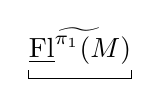
\begin{tikzpicture}[baseline=(F.base)]
\node[inner sep=0pt] (F) {$\widetilde{\underline{\mathrm{Fl}}^{\pi_1}(M)}$};
\draw ([yshift=-2pt]F.south west) -- ++(0,-3pt) -| ([yshift=-2pt]F.south east);
\end{tikzpicture}}{}^*$.
% slanted
\margin{cf plus bas \unsure{la|le} \unsure{notation} $\widetilde C$}

Pour tout cardinal $\pi\ge\pi_0$, je désigne par $M^\pi$ la sous-catégorie \inserted{str.} pleine de $M$ dont l'ens. des objets est $\mathrm{Filt}^\pi$.
\margin{$^*$ \deleted{\unsure{Etant posé}} si $C$ est une catégorie, je désigne par $\widetilde C$ l'ens. des classes d'isomorph. d'objets de $C$. \unsure{Signalons qu'on a toujours} $\mathrm{card}\,\widetilde{\underline{\mathrm{Fl}}(C)}\ge\mathrm{card}\,\deleted{\unsure{\mathrm{Ob}|C}}\widetilde C$ $^*$}
% slanted
\margin{$^*$ Car $\widetilde C\unsure{\hookrightarrow|\leftrightarrow}\widetilde{\mathrm{Fl}(C)}$ via $\unsure{\mathrm{cl}.|\mathrm{cl}}(X)\mapsto\mathrm{cl}(\mathrm{id}_X)$}

1°) Si $r\unsure{\ge|>}\mathrm{Sup}(\deleted{\unsure{\pi_0,}}\pi_{\unsure{1|0}},C_1)$, on a
\[
\mathrm{card}\left(
\underset{\substack{\Vert\\\underline{\mathrm{Fl}}(M^r)}}{
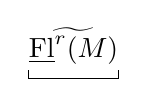
\begin{tikzpicture}[baseline=(F.base)]
\node[inner sep=0pt] (F) {$\widetilde{\underline{\mathrm{Fl}}^r(M)}$};
\draw ([yshift=-2pt]F.south west) -- ++(0,-3pt) -| ([yshift=-2pt]F.south east);
\end{tikzpicture}}
\right)\le 2^{(r^{\pi_0})}
\qquad(=2^r,\text{ si }r=2^c,\text{ avec }c\ge\unsure{r_0|\pi_0}).
\tag*{(3.7)}
\]
2°) Si $r,s\ge\mathrm{Sup}(\pi_1,\deleted{\unsure{\pi_0,}}C_1)$, et si \inserted{$A\in\mathrm{Filt}^r$,} $X\in\mathrm{Filt}^s$, on \unsure{à|a}
\[
\begin{aligned}
\mathrm{Card}\,\widetilde{\underline{\mathrm{Fl}}(M^r_{/X})}
&\le s^{(r^{\pi_0})}\quad
\left\{\begin{aligned}
&=s^r\quad\text{si }r=2^c,\text{ avec }c\ge\pi_0\\
&=s\quad\text{si }s=2^{c'},\text{ avec }c'\ge r^{\pi_0}.
\end{aligned}\right.\\
\inserted{\mathrm{Card}\,\mathrm{Hom}_M(A,X)}&\inserted{\le s^{(r^{\pi_0})}}
\end{aligned}
\tag*{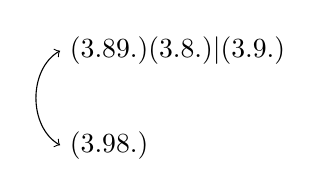
\begin{tikzpicture}[baseline=(a.base)]
\node[anchor=west] (a) at (0,0) {$(3.\deleted{\unsure{8}}9.)\deleted{\unsure{(3.8.)|(3.9.)}}$};
\node[anchor=west] (b) at (0,-1.2) {$(3.\deleted{\unsure{9}}8.)$};
\draw[<->] (a.west) to[bend right=60] (b.west);
\end{tikzpicture}}
\]
\uline{NB} Si on admet l'hypothèse du continu généralisé, qui implique que $\pi^{\pi'}=\pi$ si $\pi>\pi'$ ($\pi$ cardinal infini, $\pi'\ge1$), alors \unsure{pour} \deleted{$r\ge\mathrm{Sup}(\pi_0$} $r$ tel que $r>\pi_0$, les formules précédentes donnent (avec de plus $r\ge\mathrm{Sup}(\pi_1,C_1)$) :
\[
\mathrm{card}\,\widetilde{\underline{\mathrm{Fl}}^r(M)}\le2^r
\tag*{(3.7 bis)}
\]
\[
\begin{aligned}
\mathrm{card}\,\widetilde{\underline{\mathrm{Fl}}(M^r_{/X})}&\le s^r\qquad(\text{si }X\in\mathrm{Filt}^s).\\
\inserted{\mathrm{card}\,\mathrm{Hom}_M(A,X)}&\inserted{\le s^r\quad(\text{si }A\in\mathrm{Filt}^r,\ X\in\mathrm{Filt}^s).}
\end{aligned}
\tag*{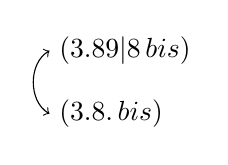
\begin{tikzpicture}[baseline=(a.base)]
\node[anchor=west] (a) at (0,0) {$(3.\deleted{\unsure{8}}\unsure{9|8}\,\text{bis})$};
\node[anchor=west] (b) at (0,-.8) {$(3.8.\,\text{bis})$};
\draw[<->] (a.west) to[bend right=60] (b.west);
\end{tikzpicture}}
\]
Sans hypothèse du continu, ces formules sont \unsure{aussi|encore} valables, pour $r$ de la forme $2^c$, avec $c\ge\unsure{r_0|\pi_0}$.
Ce sont ces \inserted{dernières} formules \deleted{\unsure{qui}} ont l'air les plus naturelles. Pour (3.8. bis), \inserted{et (3.9. bis)} je \unsure{signale|rappelle} que le $2^e$ membre $s^r$ est le cardinal de l'ens. $\mathrm{Hom}_{\mathrm{Ens}}(A,X)$, si \deleted{$\unsure{A|A_2}$} \inserted{$A,X$ sont deux ens. tels que} ($\mathrm{card}\,A=r$, $\mathrm{card}\,X=s$. On ne peut donc espérer améliorer (3.8 bis)! Pour le
% archive sheet number: 144

\scanpage{146}
\mspage{20}
\unsure{premiere|première} formule \inserted{3.\unsure{9|8}.bis}, notons que l'on a égalité lorsque $M$ est la catégorie des couples $(A,B)$, $A$ un ensemble et $B$ une partie de $A$, avec les flèches évidentes, et qu'on définit $M^\pi$ (pour $\pi\ge\unsure{\aleph_0|\pi_0}$) comme la sous-catégorie str. pleine \unsure{formée|fermée} des $(A,B)$ tels que $\mathrm{card}\,A\ge\deleted{\unsure{\aleph_0}}\pi$.

\uline{Démonstration de 3.1.} Prouvons d'abord la formule 3.8.
\[
\mathrm{card}\,\mathrm{Hom}(A,X)\le s^{(r^{\pi_0})}\qquad
\left\{\begin{aligned}
&\text{si }A\in\mathrm{Filt}^r,\ X\in\mathrm{Filt}^s\\
&r\ge\deleted{\unsure{\mathrm{Sup}(}}\pi_1,\deleted{\unsure{C_1}}),\ s\ge\mathrm{Sup}(\deleted{\unsure{\pi_0|2}}\pi_1,C_1)
\end{aligned}\right.
\]
(NB. \unsure{Je n'utiliserai|Je n'utilise} pas $r\ge C_1$, postulé dans 3.1 \uline{1°})
\deleted{\unsure{Soit} $\pi_1'=\mathrm{Sup}(\pi_0,\pi_1)$.}
\deleted{\unsure{J'écris|Il est}}
\[
\begin{aligned}
A&=\varinjlim_I A_i,\qquad\mathrm{card}\,I\le r^{\pi_0},\quad A_i\in\mathrm{Filt}^{\pi_0}\\
X&=\varinjlim_J X_j\qquad\mathrm{card}\,J\le s^{\pi_1^{\deleted{\unsure{\prime|*}}}},\quad X_j\in\mathrm{Filt}^{\pi_1^{\deleted{\unsure{\prime|*}}}}\\
&\hspace{70pt}J\text{ grand devant }\pi_1^{\deleted{\unsure{\prime|*}}},\ \deleted{\text{\unsure{plus grand|donc grand} devant }\pi}
\end{aligned}
\]
On a
\[
\mathrm{Hom}(A,X\unsure{]|)}=\varprojlim_{\unsure{i|j}\in I}
\underbrace{\mathrm{Hom}(A_i,\varinjlim_J X_j)}_{
\begin{gathered}
\unsure{\Vert|\wr}\longrightarrow
\begin{gathered}\text{car les }\unsure{A|A_i}\in\mathrm{Filt}^{\pi_0}\\\text{sont }\pi_1\text{-accessibles\unsure{;|,}}\end{gathered}\\
\varinjlim_{j\in J}\underbrace{\mathrm{Hom}(A_i,X_j)}_{\text{de cardinal }\le C_1}
\end{gathered}}
\]
donc pour $\unsure{A|\forall|\text{tt}}\ i\in I$
\[
\mathrm{Hom}(A_i,X\unsure{]|)}\le\mathrm{card}(J)\times C_1\le s^{\pi_1}\times C_1=s^{\pi_1}
\]
\margin{car $s\ge C_1$ donc $s^{\pi_1}\ge C_1$}
d'où
\[
\mathrm{card}\left(\varprojlim_{j\in I}\mathrm{Hom}(A_i,X\unsure{]|)}\right)
\le (s^{\pi_1})^{\mathrm{card}\,I}\le
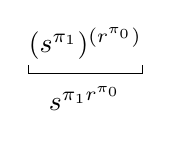
\begin{tikzpicture}[baseline=(F.base)]
\node[inner sep=0pt] (F) {$(s^{\pi_1})^{(r^{\pi_0})}$};
\draw ([yshift=-2pt]F.south west) -- ++(0,-3pt) -| ([yshift=-2pt]F.south east);
\node[below=6pt] at (F.south) {$s^{\pi_1r^{\pi_0}}$};
\end{tikzpicture}
\]
Comme $r\ge\pi_1$, on a $r^{\pi_0}\ge\pi_1$, donc $r^{\pi_0}\pi_1=r^{\pi_0}$, d'où
\[
\mathrm{card}\,\mathrm{Hom}(A,X)\le s^{(r^{\pi_0})},
\]
c'est bien la formule 3.8. Pour en tirer une estimation pour $M^r_{/X}$ (avec $X\in\mathrm{Filt}^s$),
% archive sheet number: 145

\scanpage{147}
\mspage{21}
je vais d'abord majorer le cardinal des classes d'isomorphie d'objets de $M^r_{/X}$, i.e. des \deleted{objets} flèches à isom. près (dans $M^r$)
\diagram{\begin{tikzcd}[ampersand replacement=\&,column sep=large]
A\arrow[r]\&X
\end{tikzcd}}
\margin{$X$ fixé dans $\mathrm{Filt}^s$\quad $A$ variable dans $M^r$.}
On aura
\[
A=\varinjlim_{i\in I}A_i\qquad
\begin{aligned}
&\text{avec }A_i\in\mathrm{Filt}^{\pi_0}\\
&I\text{ ens ordonné de cardinal }\le r^{\pi_0}
\end{aligned}
\]
Pour $I$ fixé, le \deleted{nombre des} cardinal de l'ensemble des systèmes inductifs indexés par $I$, dans $M^{\pi_0}_{/X}$, \deleted{est majoré par} à isom près, peut se majorer ainsi : pour \deleted{tt} $i\in I$, il faut choisir $A_i$ \inserted{dans $M^{\pi_0}$} (\deleted{dans} \unsure{seul|seule} sa classe dans $\widetilde{M^{\pi_0}}$ importe), donc choix majoré par \deleted{$\unsure{C_0|C_1}$} $\mathrm{card}\,\widetilde{M^{\pi_0}}\inserted{\le C_0}$, et pour tous les $i$, par
\[
\mathrm{card}\,I\times C_0\le r^{\pi_0}\times C_0,
\]
et \deleted{comme} \inserted{si} $r\ge C_0$, \inserted{donc $r^{\pi_0}\ge C_0$,} on a donc une majoration \deleted{\unsure{des|du}} choix possibles d'un système des \uline{objets} $A_i$ \deleted{$\unsure{i\in I|\pi}$} dans $M^\pi$, à isom près, par $r^{\pi_0}$.
% slanted
\margin{On a \unsure{pris ici} $C_0=\mathrm{card}\,\widetilde{\underline{\mathrm{Fl}}^{\pi_0}}$, donc $C_0\le C_1$}
Si on se donne de plus les morphismes de transition $A_i\mathbin{-}A_j$ pour $i\unsure{\subset|<}j$, cela fait pour chaque paire \unsure{compatibles|comparables}, \inserted{\unsure{élém.|élémts|élus}} dans $I\times I$, un choix majoré par $C_0$, donc encore une majoration par
\[
\underbrace{\mathrm{card}(I\times I)}_{=(\mathrm{card}\,I)^2=\mathrm{card}\,I}\times C_0\le r^{\pi_0}\cdot C_0=r^{\pi_0}.
\]
Donc \inserted{l'ens.} \unsure{des|les} systèmes inductifs en question, à isom près, pour $I$ fixé, sont de cardinal
\[
\le r^{\pi_0}\cdot r^{\pi_0}=r^{\pi_0}.
\]
Enfin, les \uline{\unsure{hom.|lim.}} d'un syst. inductif donné dans $X$ sont majorés par
\[
\mathrm{card}\,I\times\unsure{s|6}^{(r^{\pi_0})}
\]
(par 3.8. déjà prouvé), donc par
\[
r^{\pi_0}\cdot s^{(r^{\pi_0})}=s^{(r^{\pi_0})}\qquad(\text{puisque }r^{\pi_0}\unsure{\le|<}s^{(r^{\pi_0})}).
\]
\deleted{\unsure{Donc|D'onc} \unsure{Au total, pour $I$|pour $I$}} \inserted{Au total, pour $I$ fixé,} \inserted{l'ens.} des syst. inductifs à isom près, indexés par $I$, \unsure{à val.} dans $M^r_{/X}$, \deleted{\unsure{sont}} \unsure{\deleted{est}|est}
% archive sheet number: 146
